% =========================================================================
% LLAMIA -- EMNLP conference poster (A0 landscape, tikzposter)
% Build: latexmk -pdf poster.tex
% =========================================================================
\documentclass[25pt, a0paper, landscape, margin=0mm, innermargin=16mm,
  blockverticalspace=16mm, colspace=18mm, subcolspace=10mm]{tikzposter}

\usepackage[T1]{fontenc}
\usepackage[utf8]{inputenc}
\usepackage{newpxtext,newpxmath}   % Palatino, as in the B-LLaVA poster
\usepackage{graphicx}
\usepackage{fontawesome5}
\usepackage{xcolor}
\usepackage{enumitem}
\usepackage{qrcode}
\usepackage{booktabs}
\usepackage{amsmath}
\usepackage[hidelinks]{hyperref}
\usetikzlibrary{shadows}

% TODO: replace with the final BITW paper page URL
\newcommand{\paperurl}{https://behavior-in-the-wild.github.io/llamia}
\newcommand{\venue}{EMNLP 2026}
\newcommand{\email}{behavior-in-the-wild@googlegroups.com}

% -------------------------------------------------------------------------
% Palette: B-LLaVA slate + Adobe red accent
% -------------------------------------------------------------------------
\definecolor{slate}{RGB}{46,58,89}
\definecolor{adobered}{HTML}{EB1000}
\definecolor{inkdark}{HTML}{1F1F1F}
\definecolor{inkgray}{HTML}{5A5A5A}
\definecolor{rulegray}{HTML}{D9DCE3}

\definecolorstyle{llamiaColors}{
  \colorlet{colorOne}{slate}
  \colorlet{colorTwo}{slate}
  \colorlet{colorThree}{inkgray}
}{
  \colorlet{backgroundcolor}{white}
  \colorlet{framecolor}{rulegray}
  \colorlet{titlefgcolor}{inkdark}
  \colorlet{titlebgcolor}{white}
  \colorlet{blocktitlebgcolor}{slate}
  \colorlet{blocktitlefgcolor}{white}
  \colorlet{blockbodybgcolor}{white}
  \colorlet{blockbodyfgcolor}{inkdark}
  \colorlet{innerblocktitlebgcolor}{slate}
  \colorlet{innerblocktitlefgcolor}{white}
  \colorlet{innerblockbodybgcolor}{slate!5}
  \colorlet{innerblockbodyfgcolor}{inkdark}
  \colorlet{notefgcolor}{inkdark}
  \colorlet{notebgcolor}{white}
  \colorlet{notefrcolor}{slate}
}
\usecolorstyle{llamiaColors}

% Rounded slate title bar + separate rounded white body, both with soft shadow
\defineblockstyle{llamiaBlock}{
  titlewidthscale=1, bodywidthscale=1, titleleft,
  titleoffsetx=0pt, titleoffsety=0pt, bodyoffsetx=0mm, bodyoffsety=-8mm,
  bodyverticalshift=8mm, roundedcorners=14, linewidth=1.5pt,
  titleinnersep=9mm, bodyinnersep=0.8cm
}{
  \draw[color=framecolor, line width=\blocklinewidth, fill=blockbodybgcolor,
    rounded corners=\blockroundedcorners,
    drop shadow={shadow xshift=3mm, shadow yshift=-3mm, opacity=0.18}]
    (blockbody.south west) rectangle (blockbody.north east);
  \ifBlockHasTitle
    \fill[blocktitlebgcolor, rounded corners=\blockroundedcorners,
      drop shadow={shadow xshift=3mm, shadow yshift=-3mm, opacity=0.25}]
      (blocktitle.south west) rectangle (blocktitle.north east);
  \fi
}
\useblockstyle{llamiaBlock}
\usebackgroundstyle{Default}

% -------------------------------------------------------------------------
% Header (white, single logo row | serif title | venue + QR)
% -------------------------------------------------------------------------
\definetitlestyle{llamiaTitle}{
  width=\paperwidth, roundedcorners=0, linewidth=0pt, innersep=8mm,
  titletotopverticalspace=0mm, titlegraphictotitledistance=0pt
}{
  \fill[white] (\titleposleft,\titleposbottom) rectangle (\titleposright,\titlepostop);
  \fill[slate] (\titleposleft,\titleposbottom) rectangle
    ([yshift=-4mm]\titleposright,\titleposbottom);
}
\usetitlestyle{llamiaTitle}

\newcommand{\postertitle}{Exploring Collaboration between a Language and a Non-Language Agent}
\title{\postertitle}
\newcommand{\aff}[1]{\textsuperscript{#1}}
\author{%
  Harini~S~I\aff{1*}, Somesh~Singh\aff{1,2,3*}, Yaman~K~Singla\aff{1},
  Rajiv~Ratn~Shah\aff{2}, David~Doermann\aff{3}, Balaji~Krishnamurthy\aff{1}}
\institute{%
  \aff{1}Adobe Media and Data Science Research \quad
  \aff{2}IIIT-Delhi \quad \aff{3}SUNY at Buffalo \quad \aff{*}Equal contribution}

\newcommand{\hlogo}[1]{$\vcenter{\hbox{\includegraphics[height=3.4cm]{#1}}}$}
\settitle{%
  \noindent\begin{minipage}[c]{19.8cm}\raggedright
    \hlogo{images/adobe-logo.png}\hspace{1cm}%
    \hlogo{images/iiitd-logo.png}\hspace{1cm}%
    \hlogo{images/ub-logo-transparent.png}
  \end{minipage}\hfill%
  \begin{minipage}[c]{74cm}\centering\color{inkdark}
    {\fontsize{62}{70}\selectfont\bfseries \postertitle\par}
    \vspace{0.5cm}
    {\fontsize{42}{48}\selectfont \@author\par}
    \vspace{0.35cm}
    {\fontsize{31}{36}\selectfont\color{inkgray} \@institute\par}
  \end{minipage}\hfill%
  \begin{minipage}[c]{21cm}\raggedleft
    $\vcenter{\hbox{
\includegraphics[width=14.2cm]{images/emnlp-2026-logo.png}}}$%
    \hspace{0.7cm}%
    $\vcenter{\hbox{\qrcode[height=6cm]{\paperurl}}}$%
  \end{minipage}%
}

% Bullets as in B-LLaVA (triangles), in Adobe red
\setlist[itemize]{leftmargin=1.2em, itemsep=4pt, topsep=4pt,
  label={\color{slate}$\blacktriangleright$}}

% Token colors, as in the paper
\definecolor{StateColor}{HTML}{F94892}
\definecolor{LanguageColor}{HTML}{FF7F3F}
\definecolor{ActionColor}{HTML}{02B9F1}
\newcommand{\lang}[1]{\textcolor{LanguageColor}{\textbf{#1}}}
\newcommand{\action}[1]{\textcolor{ActionColor}{\textbf{#1}}}
\newcommand{\state}[1]{\textcolor{StateColor}{\textbf{#1}}}
\newcommand{\llamia}{\textsc{Llamia}}
\newcommand{\llamiaverb}{\textsc{Llamia-Verb}}
\newcommand{\bench}{\textsc{Llamia-Bench}}

% Schematic building blocks (verbalization / internalization figures)
\usetikzlibrary{arrows.meta}
\pgfmathdeclarerandomlist{latentcols}{{slate}{StateColor}{ActionColor}}
\tikzset{
  panel/.style={draw=slate, line width=1.8pt, rounded corners=14pt,
    fill=slate!3, drop shadow={shadow xshift=1.5mm, shadow yshift=-1.5mm,
    opacity=0.18}},
  % {cols}{rows}{cell pitch}{seed}: the engine's dense latent state
  pics/latent grid/.style n args={4}{code={
    \pgfmathsetseed{#4}
    \foreach \i in {1,...,#1} {\foreach \j in {1,...,#2} {
      \pgfmathrandomitem{\c}{latentcols}
      \pgfmathsetmacro{\o}{0.15+0.85*rnd}
      \fill[\c, fill opacity=\o, rounded corners=1.5pt]
        ({(\i-1)*#3},{(\j-1)*#3}) rectangle ++({0.85*#3},{0.85*#3});
    }}
  }},
  pics/policy bars/.style={code={
    \foreach \h [count=\i] in {1.55,1.15,0.95,0.75,0.6,0.48,0.38,0.3,0.24,0.18,0.14,0.1} {
      \fill[ActionColor, fill opacity={1-0.06*\i}] ({(\i-1)*0.36},0) rectangle ++(0.27,\h);
    }
    \draw[inkgray, line width=1pt] (-0.1,0) -- (4.3,0);
  }},
}

% Centered question / statement line
\newcommand{\keyline}[1]{%
  \begin{center}\color{slate}\large\bfseries #1\end{center}}

% Small figure caption
\newcommand{\figcap}[1]{%
  \par\vspace{0.3em}{\small\color{inkgray}#1\par}}

\tikzposterlatexaffectionproofoff
\begin{document}
\maketitle[width=\paperwidth, titletoblockverticalspace=12mm]

\begin{columns}
% =========================================================================
\column{0.27}
% =========================================================================
\block{Motivation}{
  \begin{itemize}
    \item In many important domains such as robotics and game playing,
      the strongest available agents are \textbf{not language models}.
      Their expertise lives in internal representations of policy and
      value (e.g.\ AlphaZero, RT-1).
    \item Many useful tasks need both. In chess, an engine plays far
      better than any LLM but cannot explain a move; an LLM can explain,
      but cannot play well.
  \end{itemize}
  \keyline{How can an LLM effectively collaborate with\\
    a non-language agent?}
  \begin{itemize}
    \item We study this in \textbf{chess}: strong open engines (Lc0),
      large public data, and tasks with established metrics.
  \end{itemize}
}

\block{Verbalization Is Lossy}{
  \begin{itemize}
    \item Current methods call the agent as a tool and \textbf{verbalize}
      its output into text. Only a short summary survives; the rest of
      its internal representation is lost, at every interaction step.
  \end{itemize}
  \vspace{0.2em}
  \begin{center}
  \resizebox{\linewidth}{!}{%
  \begin{tikzpicture}[
      every node/.style={align=center},
      arr/.style={-{Latex[length=5mm,width=4mm]}, line width=2.2pt, color=slate}]
    % --- Non-language agent with its rich internal state -------------------
    \draw[panel] (0,0) rectangle (9,9.4);
    \node[font=\small\bfseries, text=slate] at (4.5,8.6) {Non-Language Agent};
    \node[font=\footnotesize, text=inkgray] at (4.5,7.85)
      {\faChessKnight\; Lc0 chess engine};
    \pic at (0.75,3.35) {latent grid={6}{5}{0.8}{11}};
    \node[font=\footnotesize, text=inkgray] at (3.1,2.85) {latent state $\mathbf{h}_s$};
    \shade[bottom color=StateColor!10, top color=StateColor!85,
      rounded corners=2pt] (6.85,3.35) rectangle (7.6,7.2);
    \draw[slate, line width=1.2pt, rounded corners=2pt] (6.85,3.35) rectangle (7.6,7.2);
    \draw[inkdark, line width=2.4pt] (6.6,5.7) -- (7.85,5.7);
    \node[font=\footnotesize, text=inkgray] at (7.22,2.85) {value};
    \pic at (0.75,0.6) {policy bars};
    \node[font=\footnotesize, text=inkgray, anchor=west] at (5.3,1.2)
      {policy over\\ all moves};
    % --- Verbalization bottleneck -------------------------------------------
    \shade[left color=slate!30, right color=LanguageColor!55]
      (9,1.5) -- (15.2,4.3) -- (15.2,5.1) -- (9,7.9) -- cycle;
    \foreach \x/\y/\c/\o in {9.45/6.4/StateColor/0.75, 9.55/2.6/ActionColor/0.65,
        10.4/5.2/slate/0.6, 10.9/3.6/StateColor/0.5, 12.0/4.75/ActionColor/0.4,
        13.3/4.45/slate/0.3} {
      \fill[\c, fill opacity=\o, rounded corners=1.5pt]
        (\x,\y) rectangle ++(0.5,0.5);
    }
    \node[font=\small\bfseries, text=slate] at (12.3,7.7) {verbalization};
    % Fragments of the state that never reach the LLM
    \foreach \x/\y/\c/\o/\s in {10.3/0.6/StateColor/0.65/0.55,
        11.4/-0.05/ActionColor/0.5/0.5, 12.5/-0.5/slate/0.38/0.45,
        13.5/-0.8/StateColor/0.26/0.4, 14.4/-1.0/ActionColor/0.16/0.35} {
      \fill[\c, fill opacity=\o, rounded corners=1.5pt,
        rotate around={18*\x:(\x+0.2,\y+0.2)}] (\x,\y) rectangle ++(\s,\s);
    }
    \node[font=\footnotesize, text=adobered, anchor=west, align=left]
      at (15.0,0.1) {\faTimesCircle\; discarded:\\ other moves,\\ other lines,\\ positional features};
    % --- Text string that crosses the bottleneck --------------------------
    \fill[LanguageColor!22] (15.2,4.3) rectangle (20.6,5.1);
    \node[draw=LanguageColor, line width=1.5pt, fill=white, rounded corners=5pt,
      font=\footnotesize\ttfamily, inner sep=6pt] (txt) at (17.6,4.7) {Nf3 (+0.3)};
    \draw[arr] (txt.east) -- (20.6,4.7);
    % --- Language agent -----------------------------------------------------
    \draw[panel] (20.6,0) rectangle (29.6,9.4);
    \node[font=\small\bfseries, text=slate] at (25.1,8.6) {Language Agent};
    \node[font=\footnotesize, text=inkgray] at (25.1,7.85) {\faComments\; LLM};
    \foreach \i/\o in {0/0.3,1/0.3,2/0.3,3/1,4/1,5/0.3,6/0.3} {
      \fill[LanguageColor, fill opacity=\o, rounded corners=1.5pt]
        (21.85+\i*0.95,5.9) rectangle ++(0.75,0.75);
    }
    \node[font=\footnotesize, text=inkgray] at (25.1,5.25) {only a few text tokens};
    \node[draw=inkgray, dashed, line width=1.2pt, rounded corners=14pt,
      fill=white, font=\footnotesize\itshape, text=inkdark, inner sep=8pt,
      text width=6.6cm] at (25.1,2.4)
      {Why Nf3? What else\\ did the engine see?\\ I have to guess the rest.};
    % --- Interaction loop ---------------------------------------------------
    \draw[arr, rounded corners=18pt] (25.1,9.4) -- (25.1,10.9) -- (4.5,10.9) -- (4.5,9.4);
    \node[font=\footnotesize, fill=white, inner sep=5pt] at (14.8,10.9)
      {tool call \texttt{get\_policy(board)} \quad
       \textcolor{adobered}{\faRedo\; lossy at every step}};
  \end{tikzpicture}}
  \end{center}
}

\block{Our Approach}{
  \begin{itemize}
    \item A \textbf{language agent} (Qwen3) collaborates with a frozen
      \textbf{non-language agent} (Lc0-BT4).
    \item \textbf{Latent state internalization:} the engine's internal
      state enters the LLM as continuous \state{state tokens}, not text.
    \item RL trains the LLM to reason over \lang{language},
      \action{action} and \state{state} tokens: \textbf{\llamia}.
  \end{itemize}
  \vspace{0.2em}
  \begin{center}
  \resizebox{\linewidth}{!}{%
  \begin{tikzpicture}[
      every node/.style={align=center},
      arr/.style={-{Latex[length=5mm,width=4mm]}, line width=2.2pt, color=slate}]
    % Engine
    \draw[panel] (0,0) rectangle (8.2,6.2);
    \node[font=\small\bfseries, text=slate] at (4.1,5.45) {Non-Language Agent};
    \node[font=\footnotesize, text=inkgray] at (4.1,4.75) {\faChessKnight\; Lc0};
    \pic at (1.35,0.55) {latent grid={8}{5}{0.7}{11}};
    % Projector
    \draw[arr] (8.2,3.1) -- node[above, font=\footnotesize, text=inkgray]
      {$\mathbf{h}_s$} (9.4,3.1);
    \shade[left color=StateColor!15, right color=StateColor!45]
      (9.4,2.2) -- (12.2,1.3) -- (12.2,4.9) -- (9.4,4.0) -- cycle;
    \draw[StateColor!80!black, line width=1.4pt, line join=round]
      (9.4,2.2) -- (12.2,1.3) -- (12.2,4.9) -- (9.4,4.0) -- cycle;
    \node[font=\footnotesize\bfseries, text=inkdark] at (10.8,3.1) {Latent\\Bridge};
    % State tokens
    \foreach \i in {0,...,6} {
      \fill[StateColor, rounded corners=1.5pt] (12.7,1.0+\i*0.62) rectangle ++(0.75,0.5);
    }
    \node[font=\footnotesize, text=StateColor!80!black] at (13.1,0.45) {$k{=}32$};
    \draw[arr] (13.55,3.1) -- (14.6,3.1);
    % LLM with interleaved language / action / state tokens
    \draw[panel] (14.6,0) rectangle (29.6,6.2);
    \node[font=\small\bfseries, text=slate] at (22.1,5.45) {Language Agent};
    \node[font=\footnotesize, text=inkgray] at (22.1,4.75) {\faComments\; LLM};
    \foreach \c [count=\i] in {LanguageColor,LanguageColor,LanguageColor,ActionColor,
        StateColor,StateColor,StateColor,StateColor,LanguageColor,LanguageColor,
        ActionColor,StateColor,StateColor,StateColor,StateColor,LanguageColor} {
      \fill[\c, rounded corners=1.5pt] ({15.4+(\i-1)*0.85},2.9) rectangle ++(0.68,0.95);
    }
    \node[font=\footnotesize, text=inkgray] at (22.1,1.9)
      {reasons over \lang{language}, \action{action}, \state{state} tokens};
    \node[font=\footnotesize\bfseries, text=slate] at (22.1,0.9)
      {the full engine state reaches the LLM};
  \end{tikzpicture}}
  \end{center}
}

% =========================================================================
\column{0.40}
% =========================================================================
\block{Latent State Internalization}{
  \begin{center}
    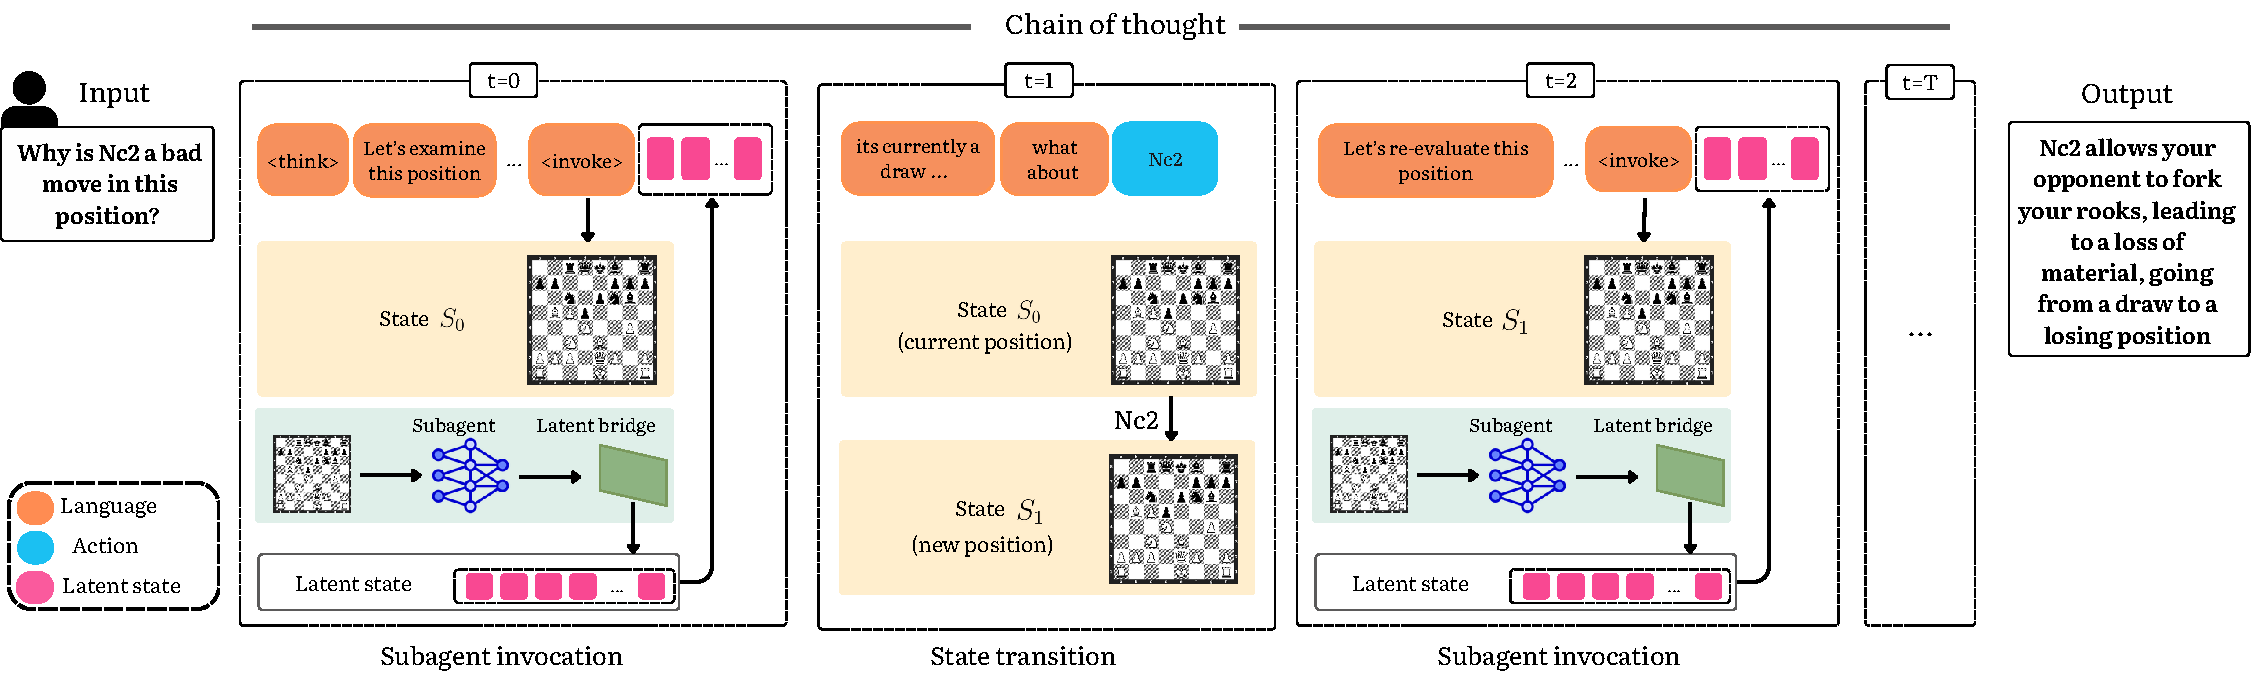
\includegraphics[width=\linewidth]{plots/llamia-fig (12).pdf}
  \end{center}
  \figcap{A single chain of thought. The LLM reasons in \lang{language},
    calls the engine on the current board, plays an \action{action} that
    changes the board, and calls the engine again on the new board.}
  \vspace{0.6em}
  \begin{itemize}
    \item \textbf{Projection.} Lc0's hidden state
      $\mathbf{h}_s \in \mathbb{R}^{1024}$ (layer 14 of 15) is mapped by a
      3-layer MLP, the \textbf{LatentBridge}, to $k{=}32$ \state{state
      tokens} in the LLM's embedding space:
      $\;\mathbf{z}_s = H_\varphi(\mathbf{h}_s) \in \mathbb{R}^{k\times e}$.
    \item \textbf{Dynamic invocation.} Inside its chain of thought, the LLM
      can play moves that update the board (including hypothetical
      moves) and call \texttt{get\_policy} on any position. Each call
      re-encodes the current state, so the LLM always reasons over the
      position it is analyzing.
    \item The LLM decides \textbf{when} to call the engine; the call is part
      of its action space.
  \end{itemize}
}

\block{Training}{
  \begin{minipage}[t]{0.50\linewidth}
    \begin{itemize}
      \item \textbf{Stage 1: projector alignment.} Only the LatentBridge
        is trained, with the LLM frozen, on engine state--policy pairs
        (predict the engine's move from the \state{state tokens}).
      \item \textbf{Stage 2: reinforcement learning.} The LLM and
        LatentBridge are trained jointly with \textbf{DAPO}. The reward is
        each task's metric. \state{State tokens} are masked from the
        policy gradient.
      \item The engine stays frozen throughout.
      \item \textbf{Control:} \llamiaverb{} uses the same LLM, engine,
        data and RL recipe, but receives the engine's output only as
        text.
    \end{itemize}
  \end{minipage}\hfill
  \begin{minipage}[t]{0.46\linewidth}
    \vspace{0pt}\centering
    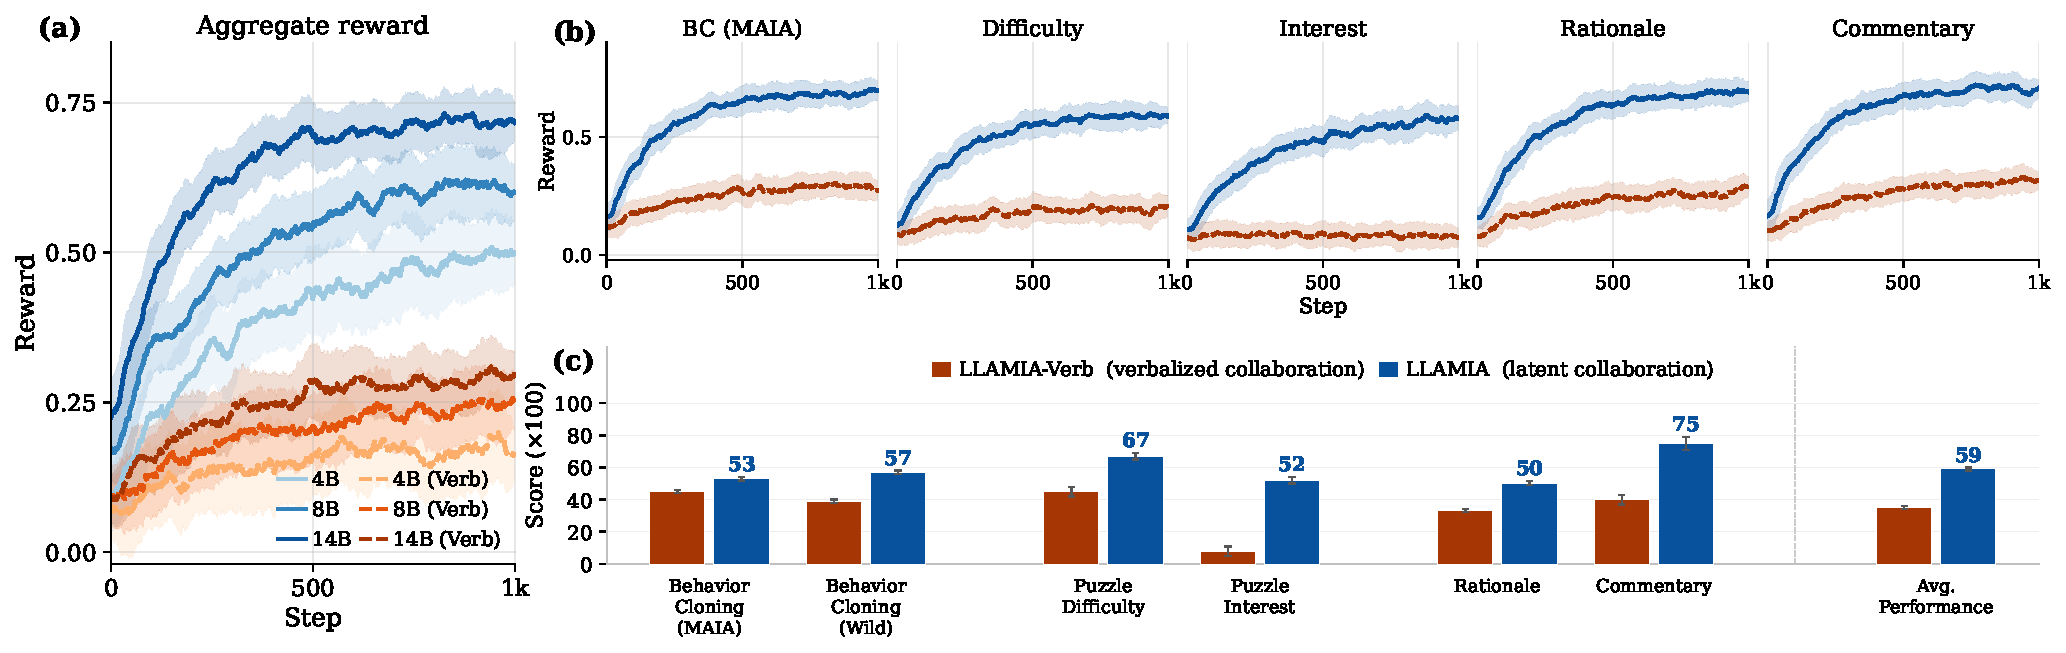
\includegraphics[width=0.92\linewidth, trim=0 0 742 0, clip]
      {plots/combined_training_bench_verb_vs_llamia.pdf}
    \figcap{Aggregate reward during DAPO training at three LLM sizes.
      Solid: \llamia{} (latent); dashed: \llamiaverb{} (text).}
  \end{minipage}
  \vspace{0.6em}
  \begin{itemize}
    \item The method works at \textbf{4B, 8B and 14B}; larger LLMs reach
      higher reward.
    \item At every size, \llamia{} trains well above \llamiaverb{}, and
      the gap grows during training, reaching \textbf{2--3$\times$} at
      the end.
    \item Scaling the LLM does not close the gap: \llamia-4B ends above
      \llamiaverb-14B.
  \end{itemize}
}

% =========================================================================
\column{0.33}
% =========================================================================
\block{\bench}{
  A suite of six collaborative chess tasks. None can be solved well by
  the LLM or the engine alone.
  \vspace{0.4em}
  \begin{center}
  \small
  \renewcommand{\arraystretch}{1.15}
  \begin{tabular}{@{}lll@{}}
    \toprule
    \textbf{Task} & \textbf{Goal} & \textbf{Metric} \\
    \midrule
    Behavior cloning (Maia) & Predict a human's move at a given rating & Move match \\
    Behavior cloning (Wild) & Same, on GM, low-time, rating-gap games & Move match \\
    Puzzle difficulty & Rank puzzles by difficulty & Spearman $\rho$ \\
    Puzzle interest & Rank puzzles by how interesting they are & Spearman $\rho$ \\
    Move rationale & Explain why a move was played & BLEU-2 \\
    Game commentary & Narrate a full game (Agadmator-2K, new) & G-Eval \\
    \bottomrule
  \end{tabular}
  \end{center}
}

\block{Results}{
  \begin{center}
    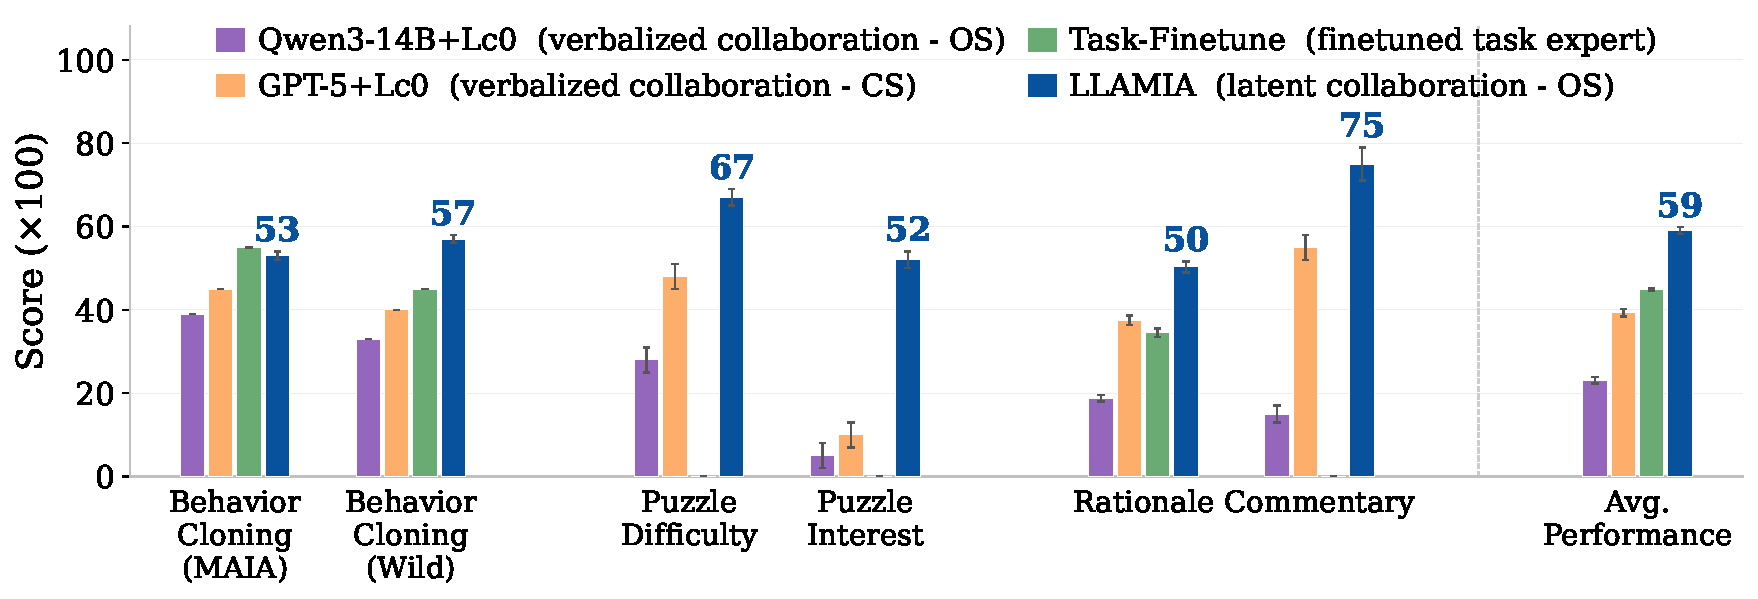
\includegraphics[width=\linewidth]{plots/panel_c_no_verb.pdf}
  \end{center}
  \begin{itemize}
    \item A single \llamia-14B model is best on all six tasks, ahead of
      GPT-5 with the same engine as a tool and of task-specific
      finetuned models.
    \item On Puzzle Interest, every text-based system scores
      ${\leq}\,12$; \llamia{} scores \textbf{52}.
  \end{itemize}
}

\block{Further Findings}{
  \begin{itemize}
    \item \textbf{The gain comes from the engine's state.} A raw board
      encoder or shuffled state tokens give no gain over text.
    \item \textbf{How the engine is used.} \llamiaverb{} mostly copies the
      engine's top move (62--76\%). \llamia{} uses different strategies
      per task, e.g.\ querying hypothetical moves for commentary.
    \item \textbf{Cost.} \llamia{} makes fewer engine calls (1.9 vs.\ 2.9
      per query); inference cost is about the same.
    \item \textbf{Human study} ($n{=}12$, rated ${\geq}1700$). Players
      spotted \llamia{} as a bot in 39\% of games (\llamiaverb: 72\%);
      72\% of commentary judgments preferred \llamia.
    \item \textbf{Beyond chess.} On Go with KataGo, the same method is
      ${\sim}10$ points above the text-based control.
  \end{itemize}
}
\end{columns}

\end{document}
